\documentclass[a4paper,12pt]{article} 

%Гралусы
\usepackage{gensymb}

%Система единиц СИ
\usepackage{siunitx}

%Добавляет возможность искать и копировать текст
\usepackage{cmap}

%Убирает пробел между названием таблицы/рисунка и самой таблицей/рисунком
\usepackage{caption}
\captionsetup[table]{skip= -0 cm}
\captionsetup[figure]{skip= -0 cm}

%Выравнивание названия таблиц по левому краю
%\usepackage[nooneline]{caption} 
%Размеры отступов 
\usepackage[left=20mm, top=20mm, right=20mm, bottom=20mm, footskip=10mm]{geometry}

%Рисунки
\usepackage{graphicx}
\usepackage{wrapfig} %обтекание элементов
\graphicspath{{graphs}{figures}}  % папки с картинками

%Русский язык в формулах
%\usepackage{mathtext}

%  Русский язык
\usepackage[T2A]{fontenc}			
\usepackage[utf8]{inputenc}			
\usepackage[english,russian]{babel}	

%Готические буквы
\usepackage{amssymb}

%Русский язык в формулах
\usepackage{mathtext}

% Математика
\usepackage{amsmath,amsfonts,amssymb,amsthm,mathtools} 
\usepackage{wasysym}

%Цветные подписи в таблице
\usepackage[table,xcdraw]{xcolor}

\usepackage{fancyhdr} % Колонтитулы
 	\pagestyle{fancy}
 	\renewcommand{\headrulewidth}{0.3mm}  % Толщина линейки, отчеркивающей верхний колонтитул
 	%\lfoot{Нижний левый}
 	%\rfoot{Нижний правый}
 	\rhead{Кафедра квантовой электроники}
 	%\chead{Верхний в центре}
 	\lhead{Белостоцкий А.И}
 	% \cfoot{Нижний в центре} % По умолчанию здесь номер страницы
 	
\begin{document} 

%Титульник 
\begin{titlepage}
	\begin{center}
		\large 	МИНИСТЕРСТВО ОБРАЗОВАНИЯ И НАУКИ РОССИЙСКОЙ ФЕДЕРАЦИИ\\
				МОСКОВСКИЙ ФИЗИКО-ТЕХНИЧЕСКИЙ ИНСТИТУТ \\
				(НАЦИОНАЛЬНЫЙ ИССЛЕДОВАТЕЛЬСКИЙ УНИВЕРСИТЕТ)\\ 
				ФИЗТЕХ-ШКОЛА ЭЛЕКТРОНИКИ, ФОТОНИКИ \\
				И МОЛЕКУЛЯРНОЙ ФИЗИКИ \\
		
		
		\vspace{4.0 cm}
		\LARGE{Отчет по лабораторной работе} \\ 
		\LARGE \textbf{Пространственные характеристики излучения полупроводникового инжекционного лазера} \\
	\end{center}
	\vspace{3 cm} \large

	%Надо подумать как это нормально написать	
	\begin{flushleft}
		Работу выполнил \hspace{5.5cm}  \underline{\hspace{3cm}} А.И.Белостоцкий \\	
		\vspace{2cm}
		Работу принял, оценка \hspace{4.3cm} \underline{\hspace{3cm}}
	\end{flushleft}
	
	
	\vfill

	\begin{center}
	Долгопрудный, 2023 г.
	\end{center}
\end{titlepage}           

\tableofcontents

\newpage

\section{Аннотация}

Инжекционным полупроводниковым лазерам (ИПЛ) свойственна миниатюрность, возможность высокочастотного управления световым сигналом за счет модуляции тока накачки, высокий дифференциальный КПД, небольшая потребляемая мощность. Это делает их весьма перспективными для волоконно-оптической связи, ЭВМ и многих других областей. 
   
В данной работе будут рассмотрены ватт-ваттная и спектральная характеристики излучения ПИЛ и светодиодов.
 
\section{Ход работы}

\subsection{Измерение ватт-ваттной характеристики ПИЛ и светодиодов12}

Меняя мощность накачки, будем измерять мощность излучения лазера и светодиодов. По полученным данным построим графики:

\begin{figure}[h!]
	\centering
	\includegraphics[width = 0.8\linewidth]{laser_vatt}
	\caption{Ватт-ваттная характеристика ПИЛ}
\end{figure}

\newpage

\begin{figure}[h!]
	\centering
	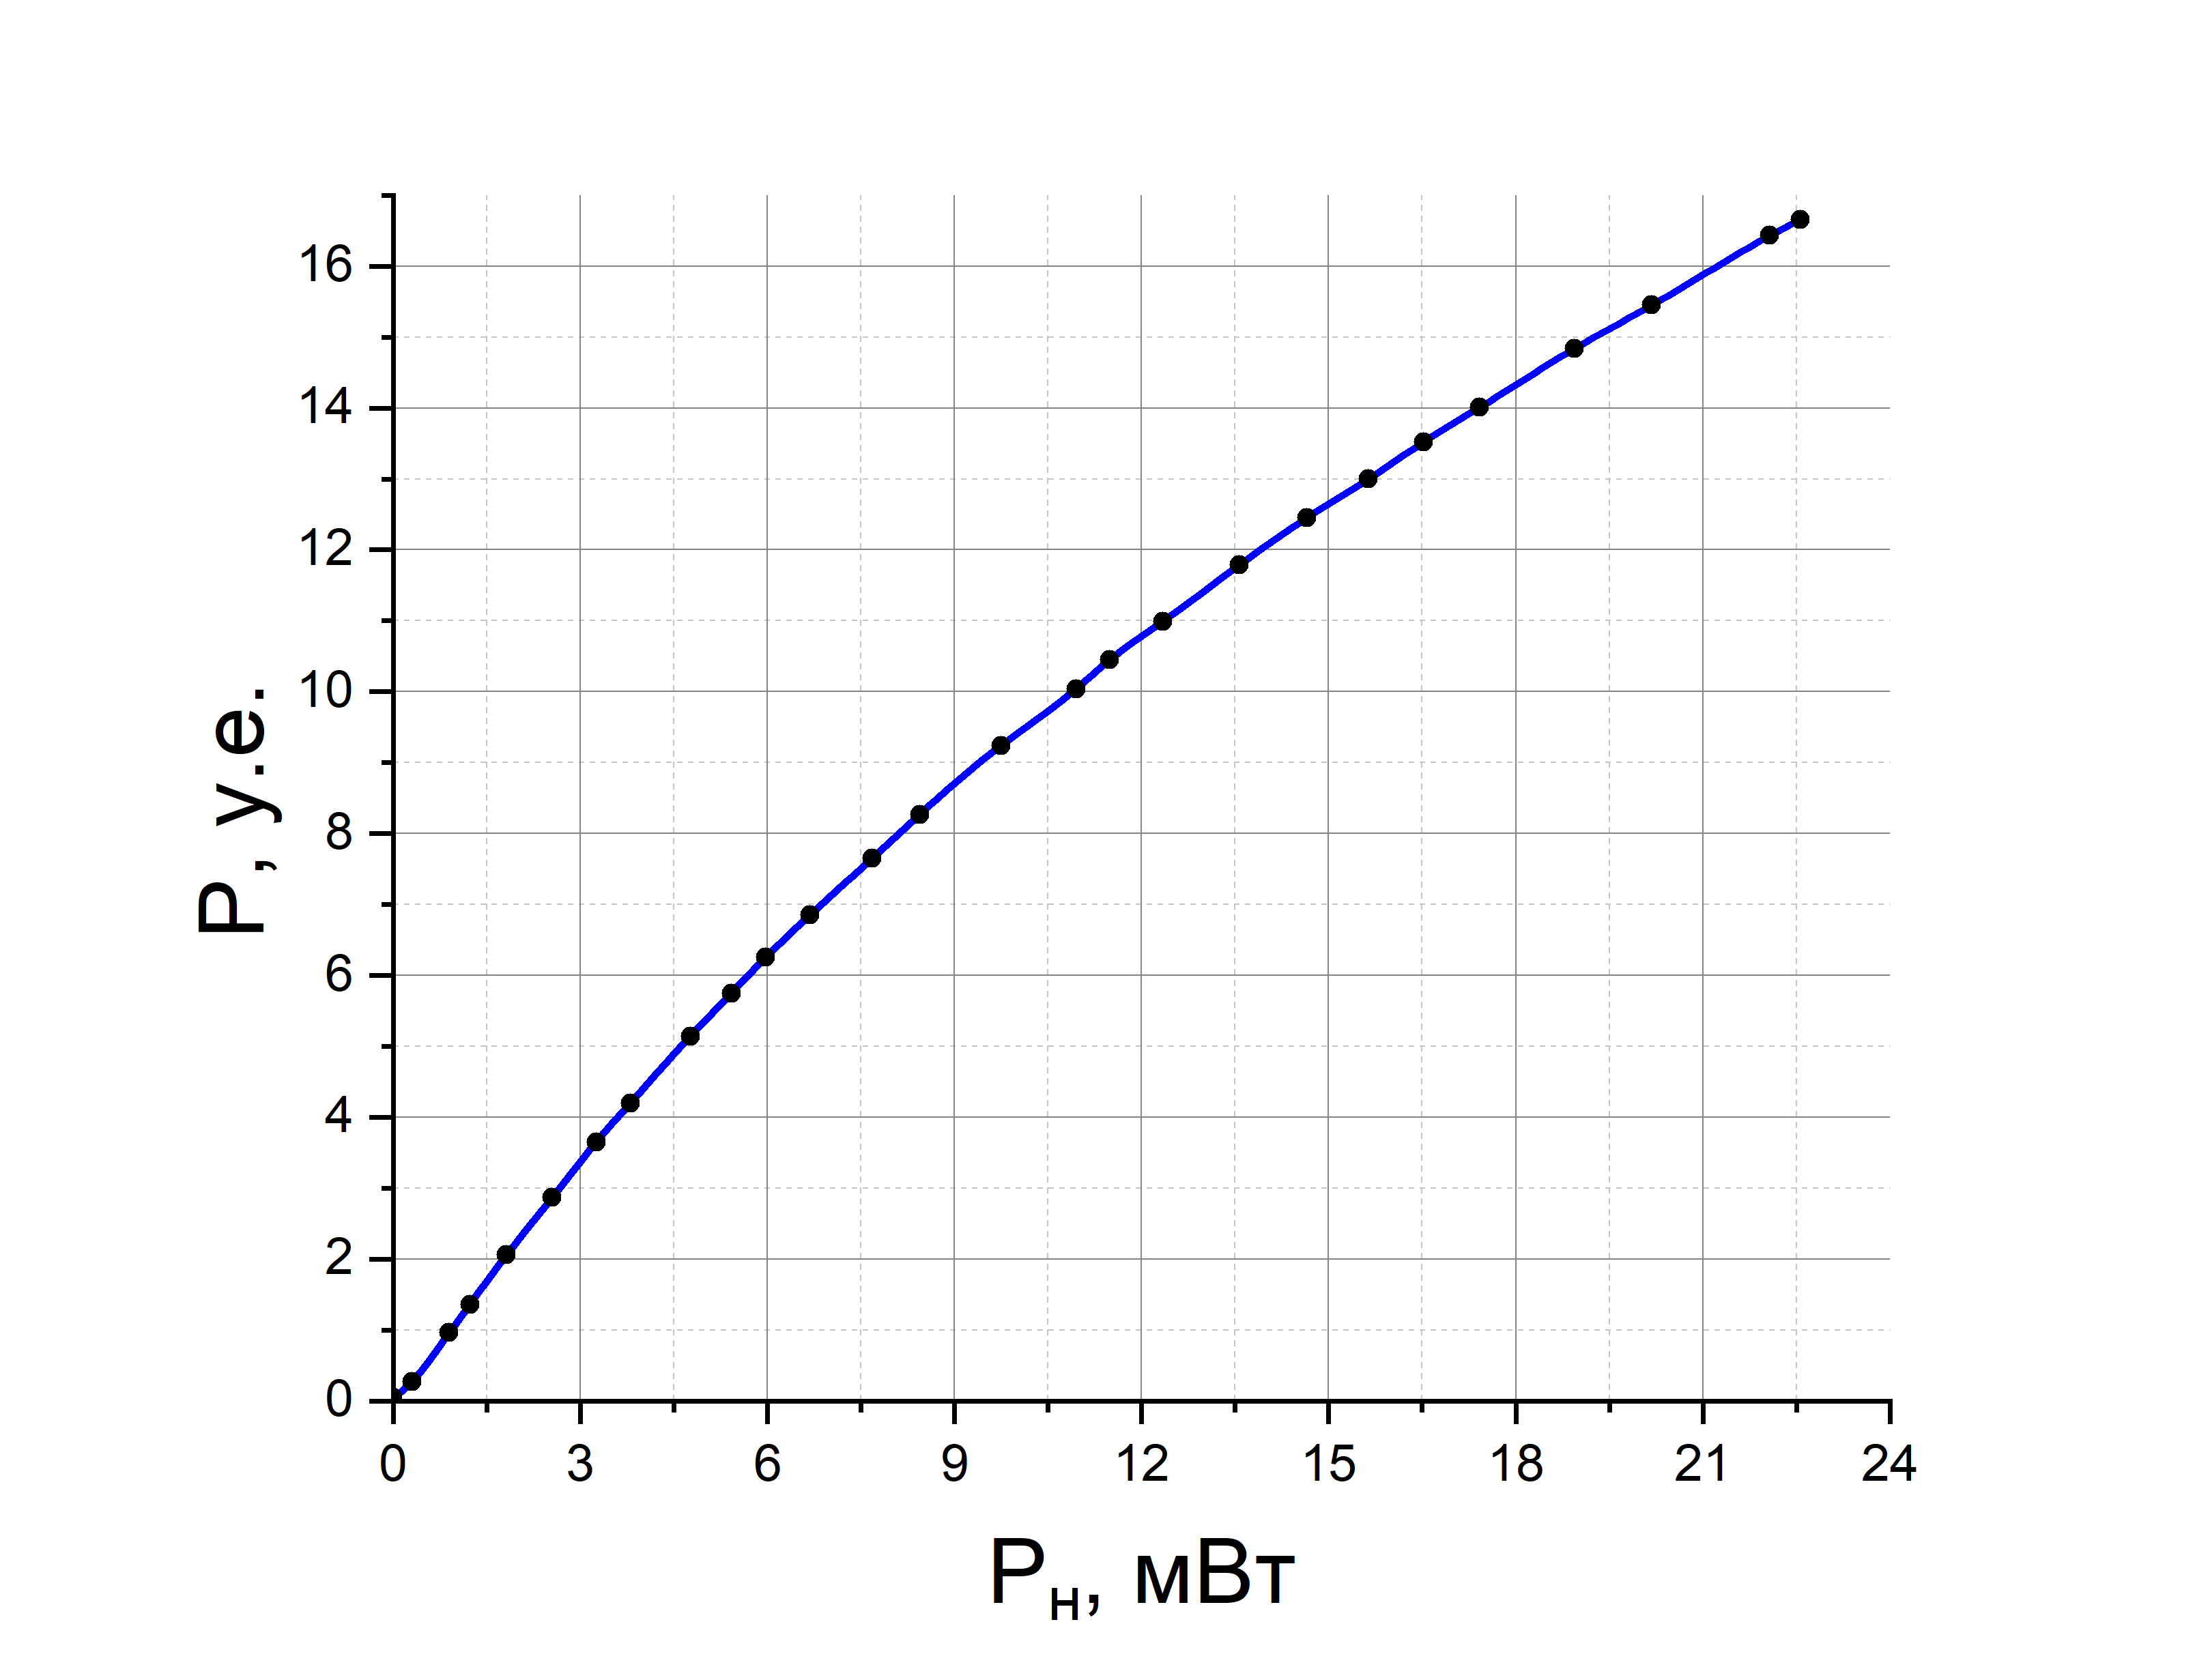
\includegraphics[width = 0.8\linewidth]{blue_vatt}
	\caption{Ватт-ваттная характеристика синего светодиода}
\end{figure}


\begin{figure}[h!]
	\centering
	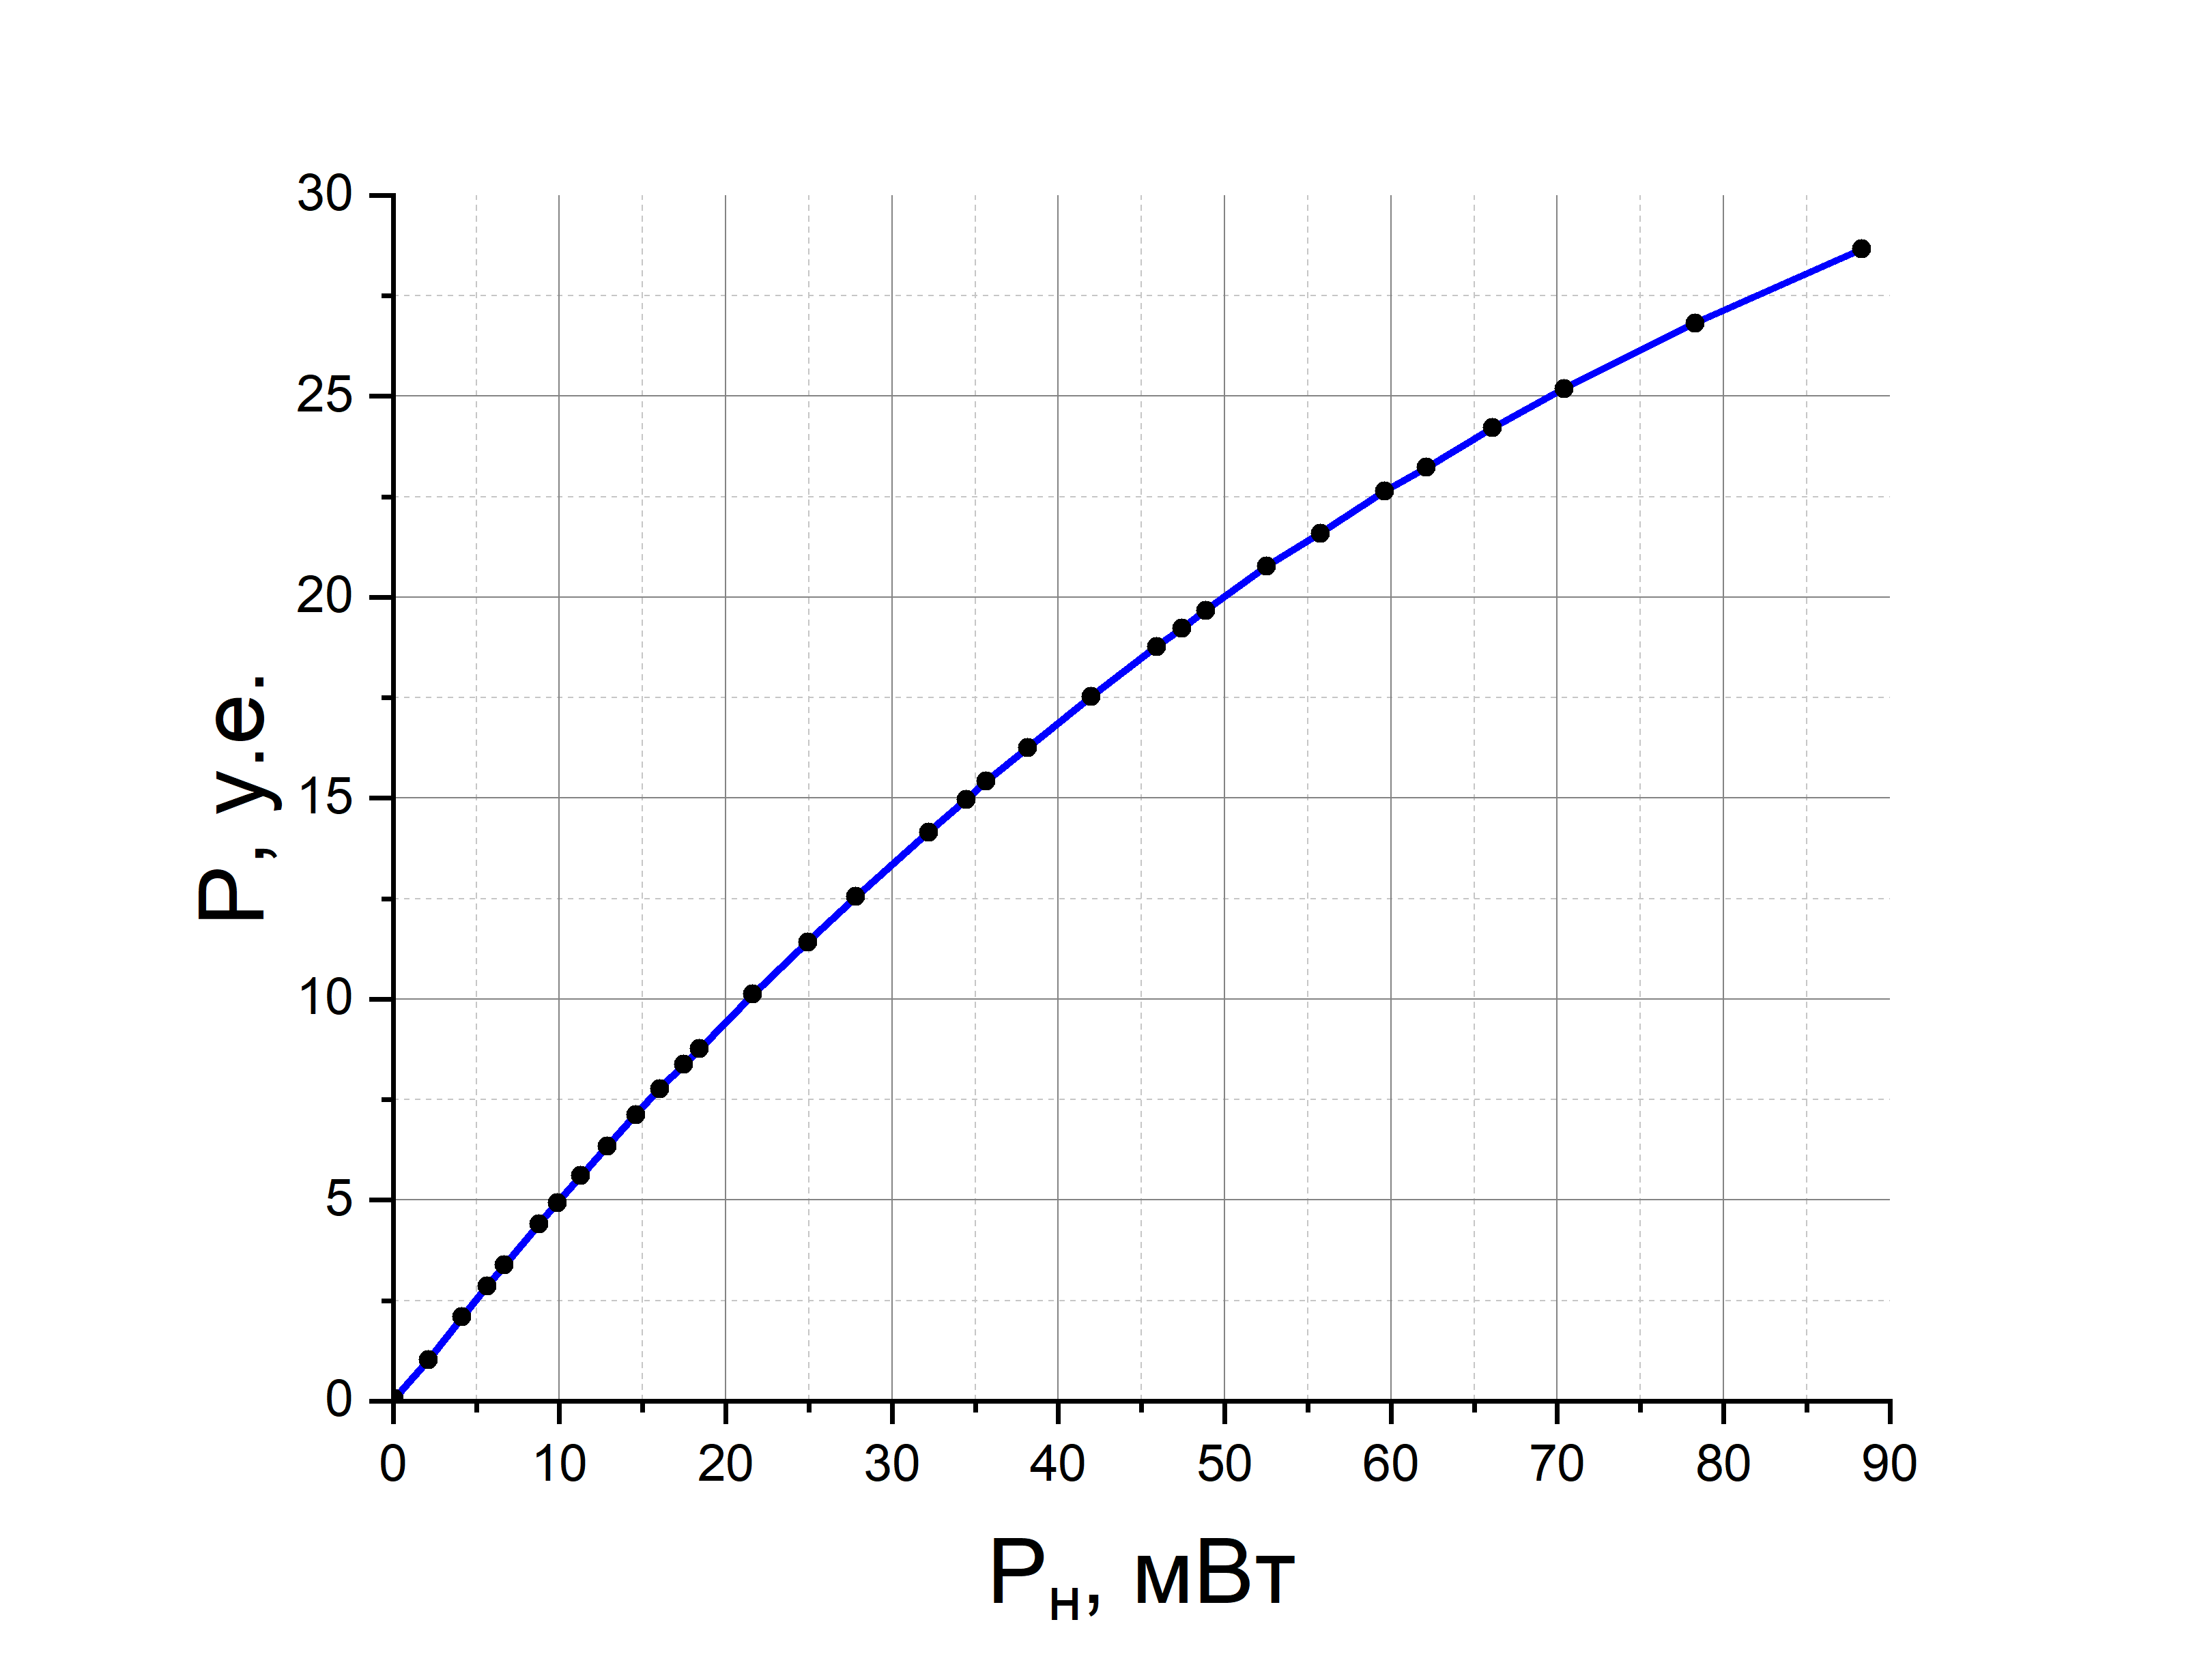
\includegraphics[width = 0.8\linewidth]{red_vatt}
	\caption{Ватт-ваттная характеристика красного светодиода}
\end{figure}

\newpage


\begin{figure}[h!]
	\centering
	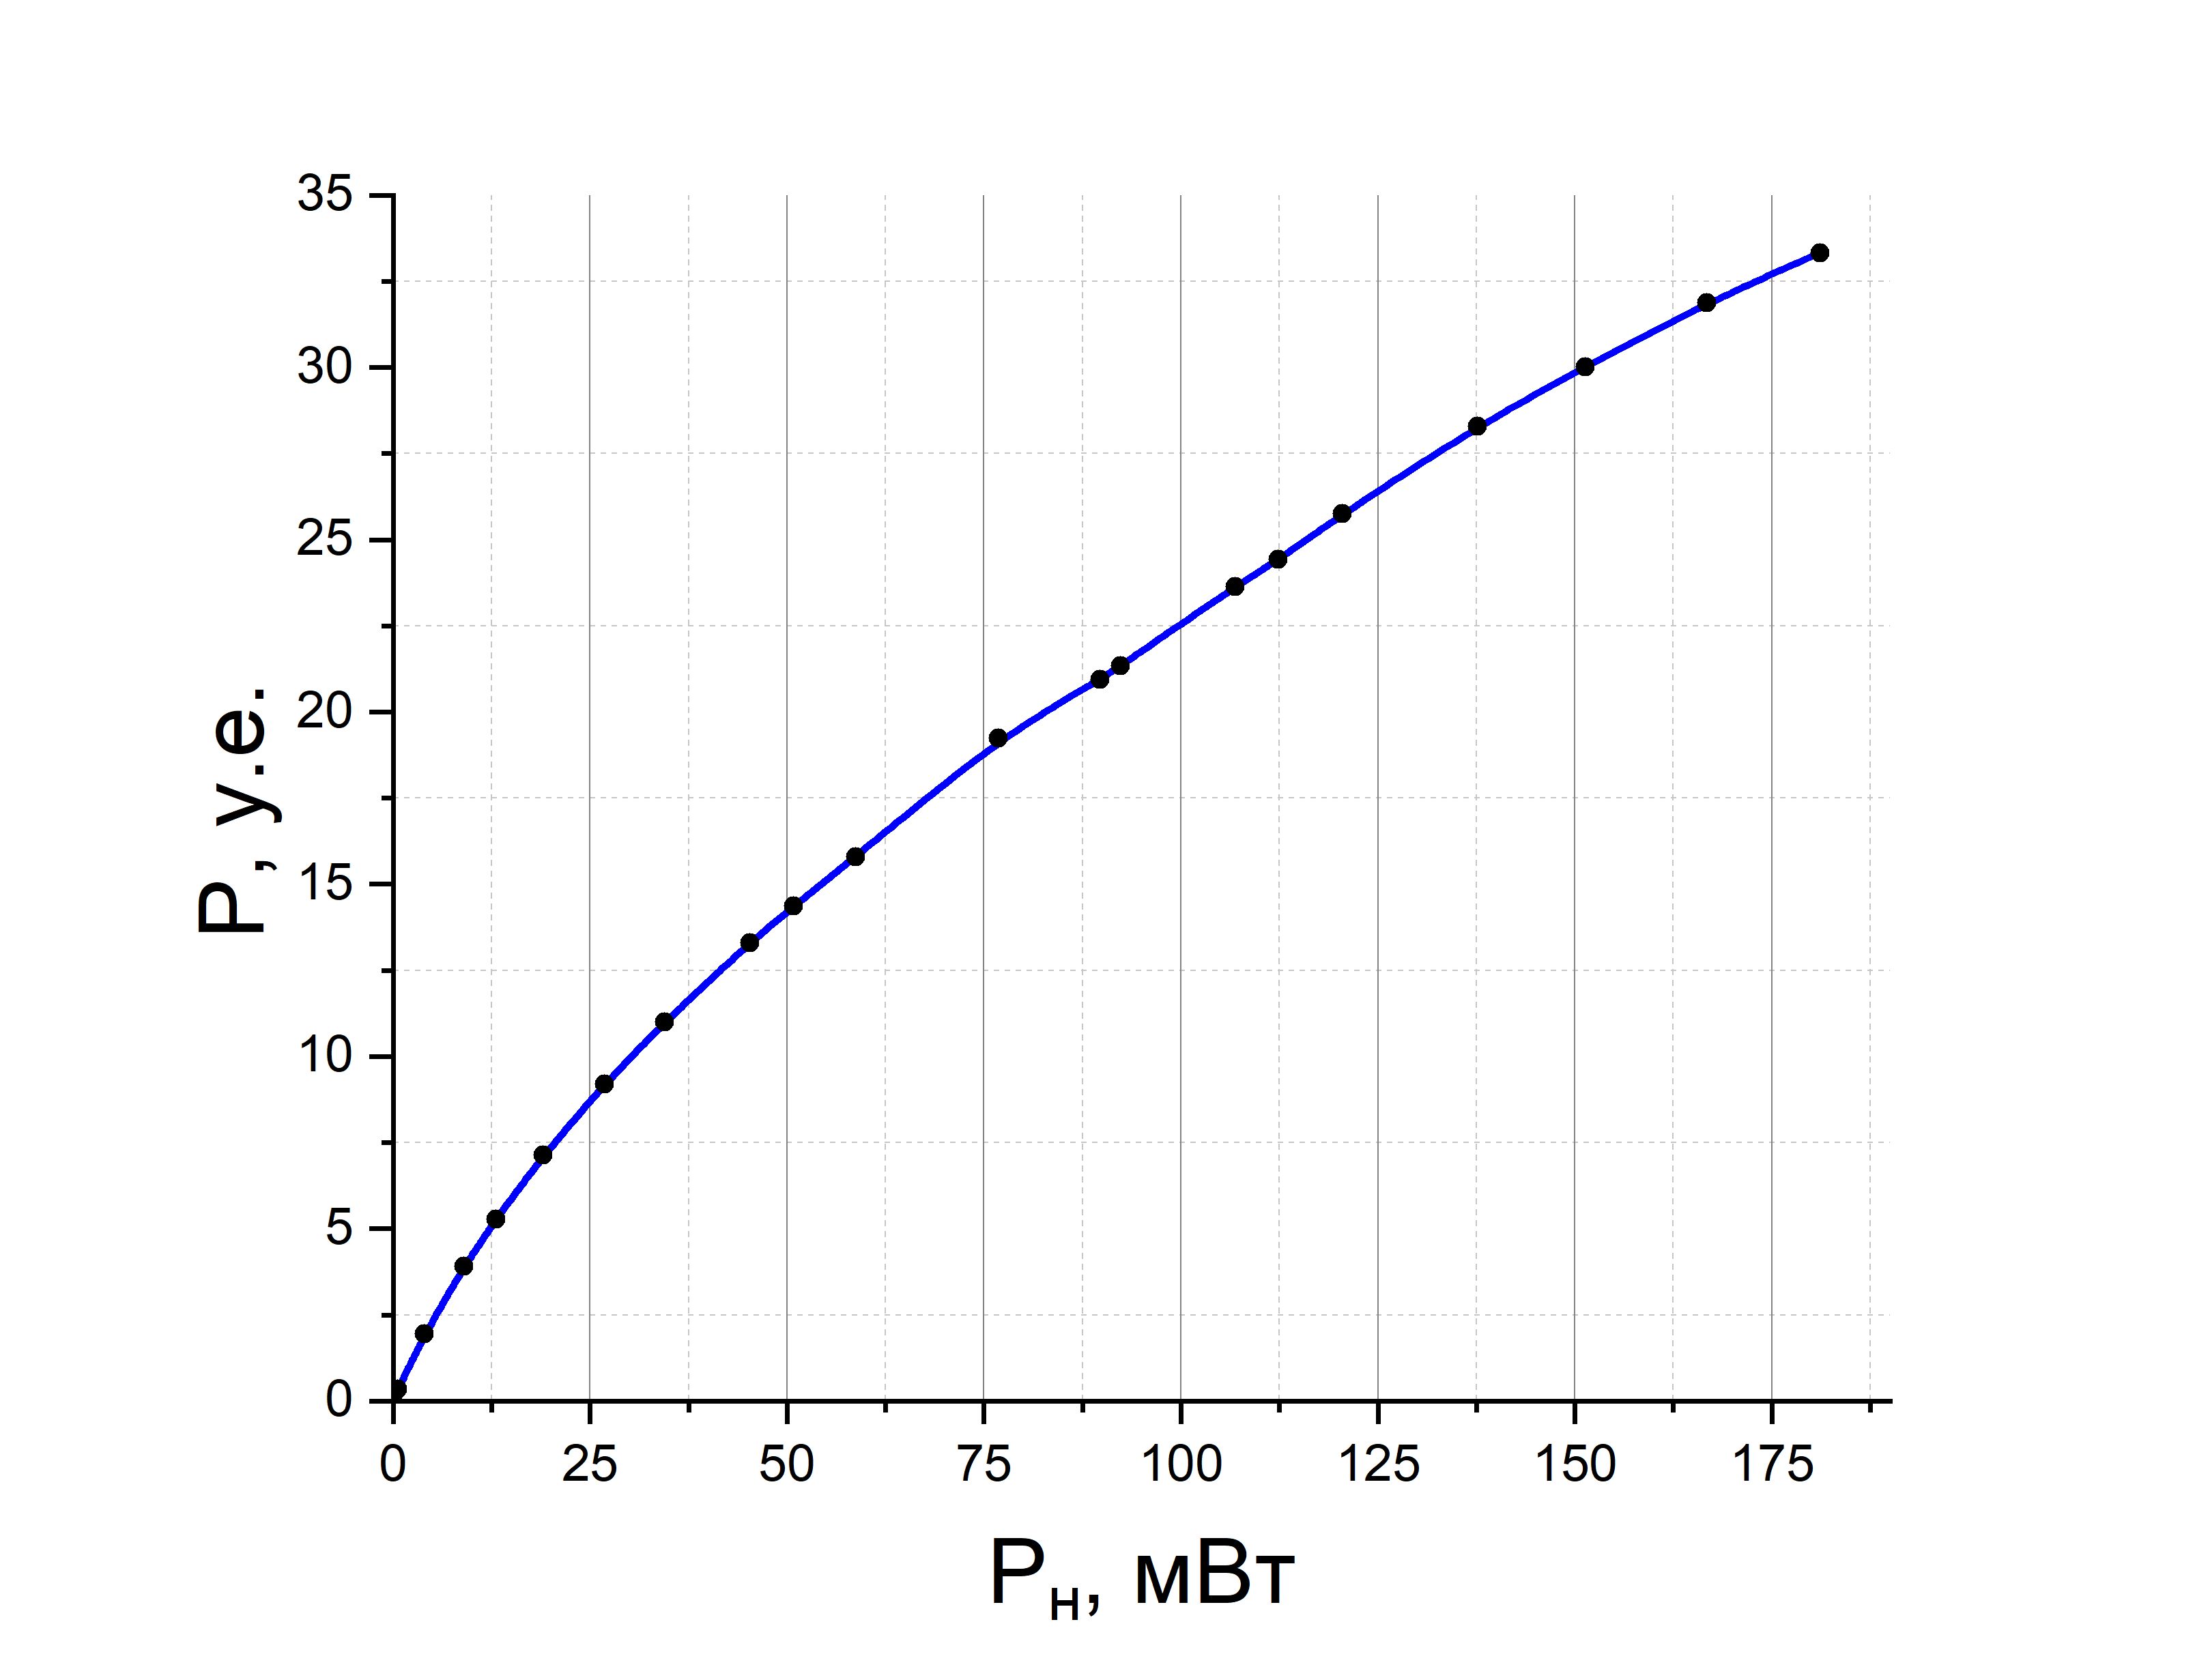
\includegraphics[width = 0.7\linewidth]{green_vatt}
	\caption{Ватт-ваттная характеристика зеленого светодиода}
\end{figure}

По ватт-ваттной характеристике ПИЛ определим пороговую мощность накачки -- аппроксимируя часть зависимости прямой определим точку пересечения с осью мощности накачки. Получим $P_{\text{порог}} \approx 32$ мВт

\subsection{Измерение спектральной характеристики ПИЛ и светодиодов}

Измерим спектральные характеристики ПИЛ и светодиодов при разных токах накачки. По результатам измерений построим графики:

\begin{figure}[h!]
	\centering
	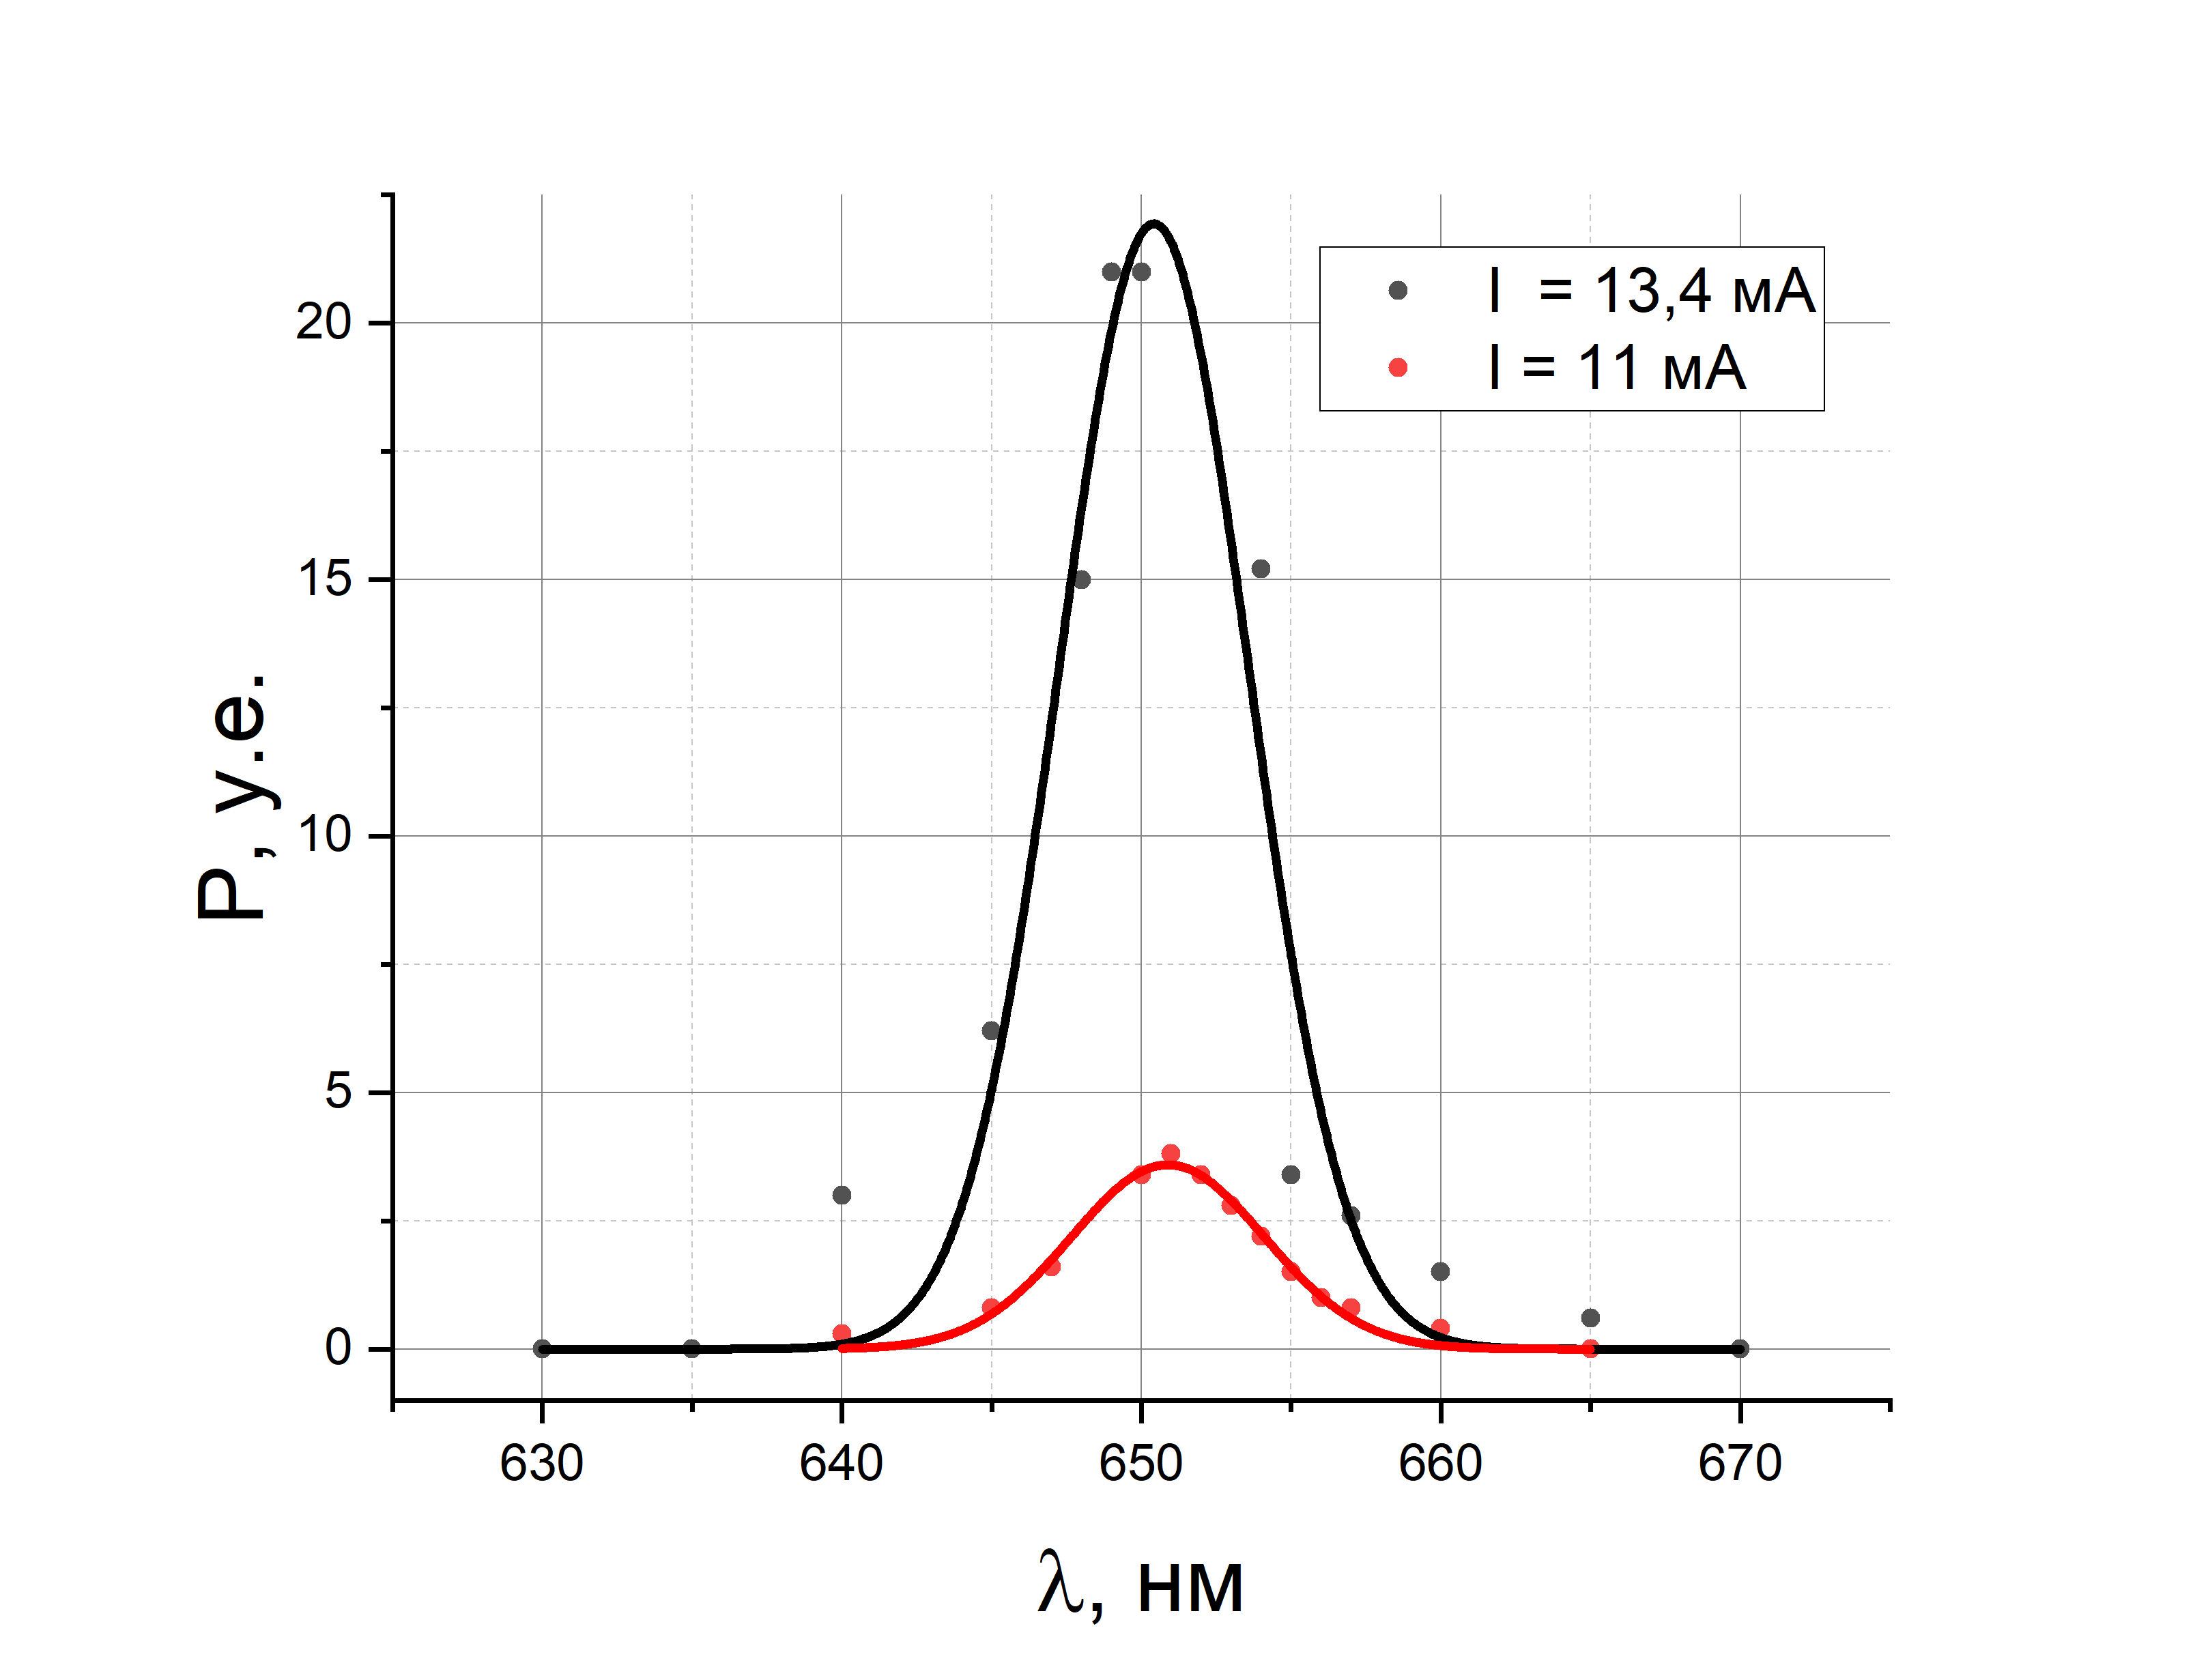
\includegraphics[width = 0.7\linewidth]{laser_1_and_2}
	\caption{Спектральная характеристика для ПИЛ при двух различных токах накачки}
\end{figure}

\newpage

\begin{figure}[h!]
	\centering
	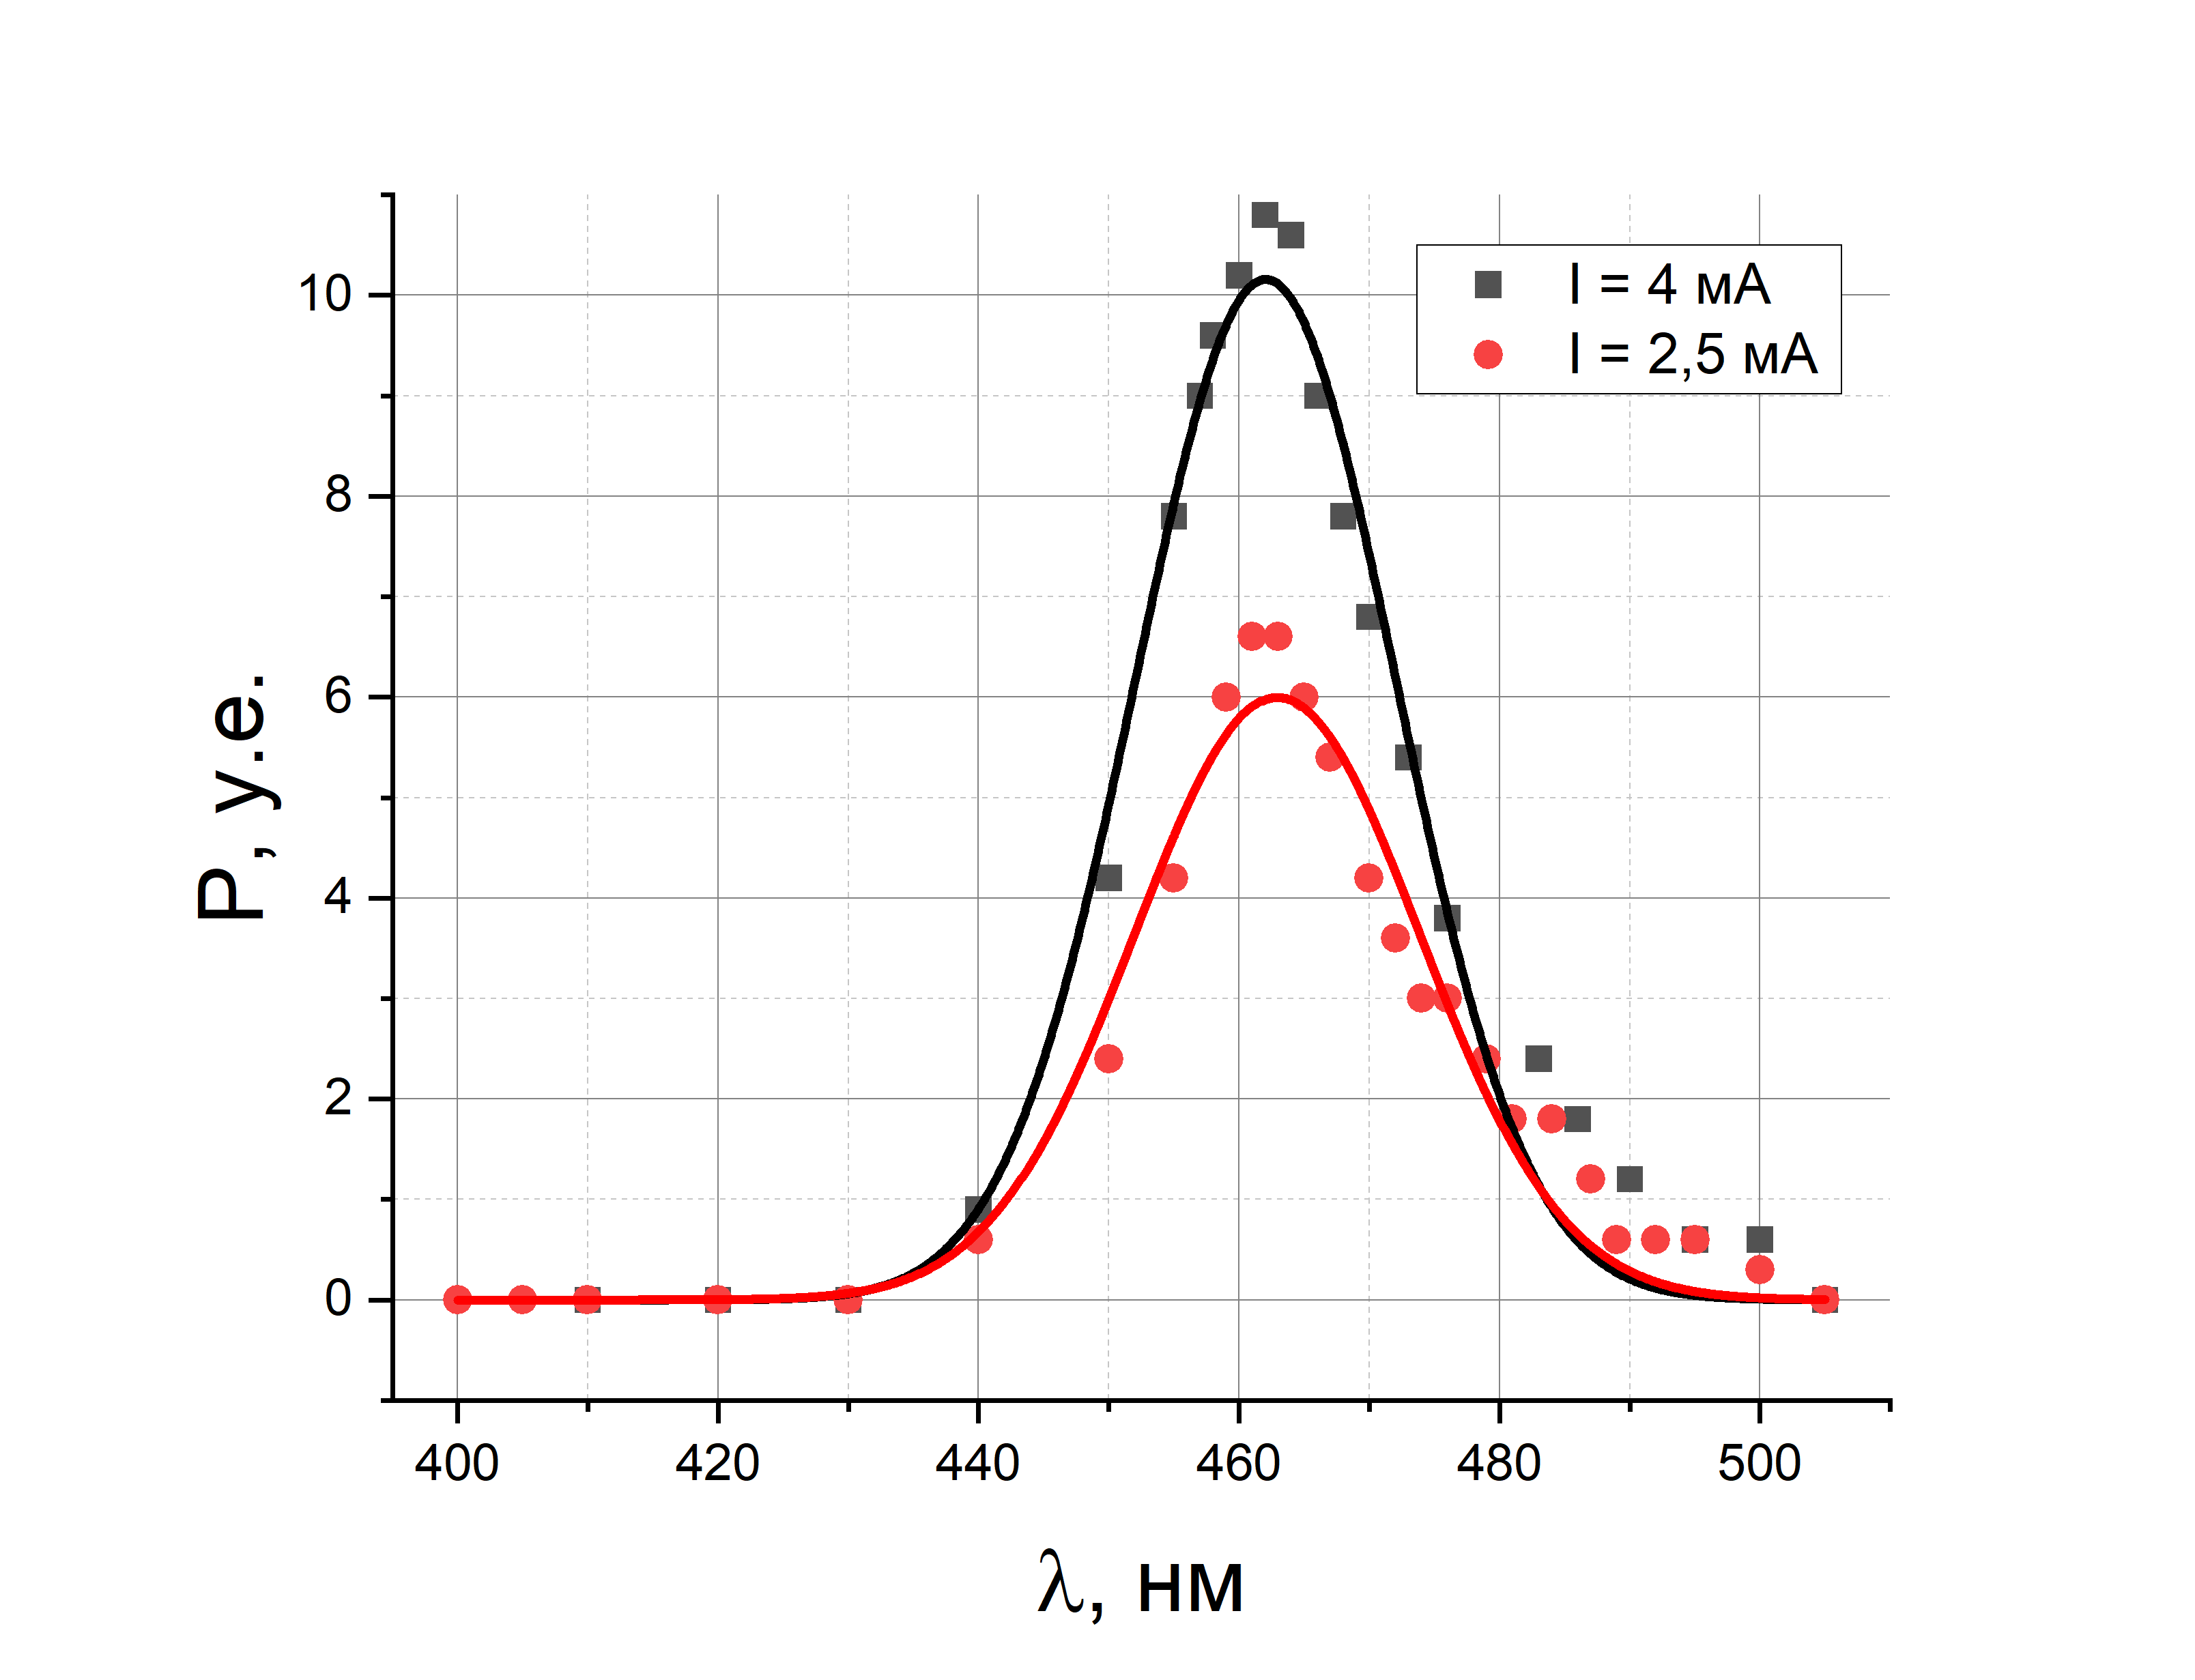
\includegraphics[width = 0.8\linewidth]{blue_1_and_2}
	\caption{Спектральная характеристика для синего светодиода при двух различных токах накачки}
\end{figure}

\begin{figure}[h!]
	\centering
	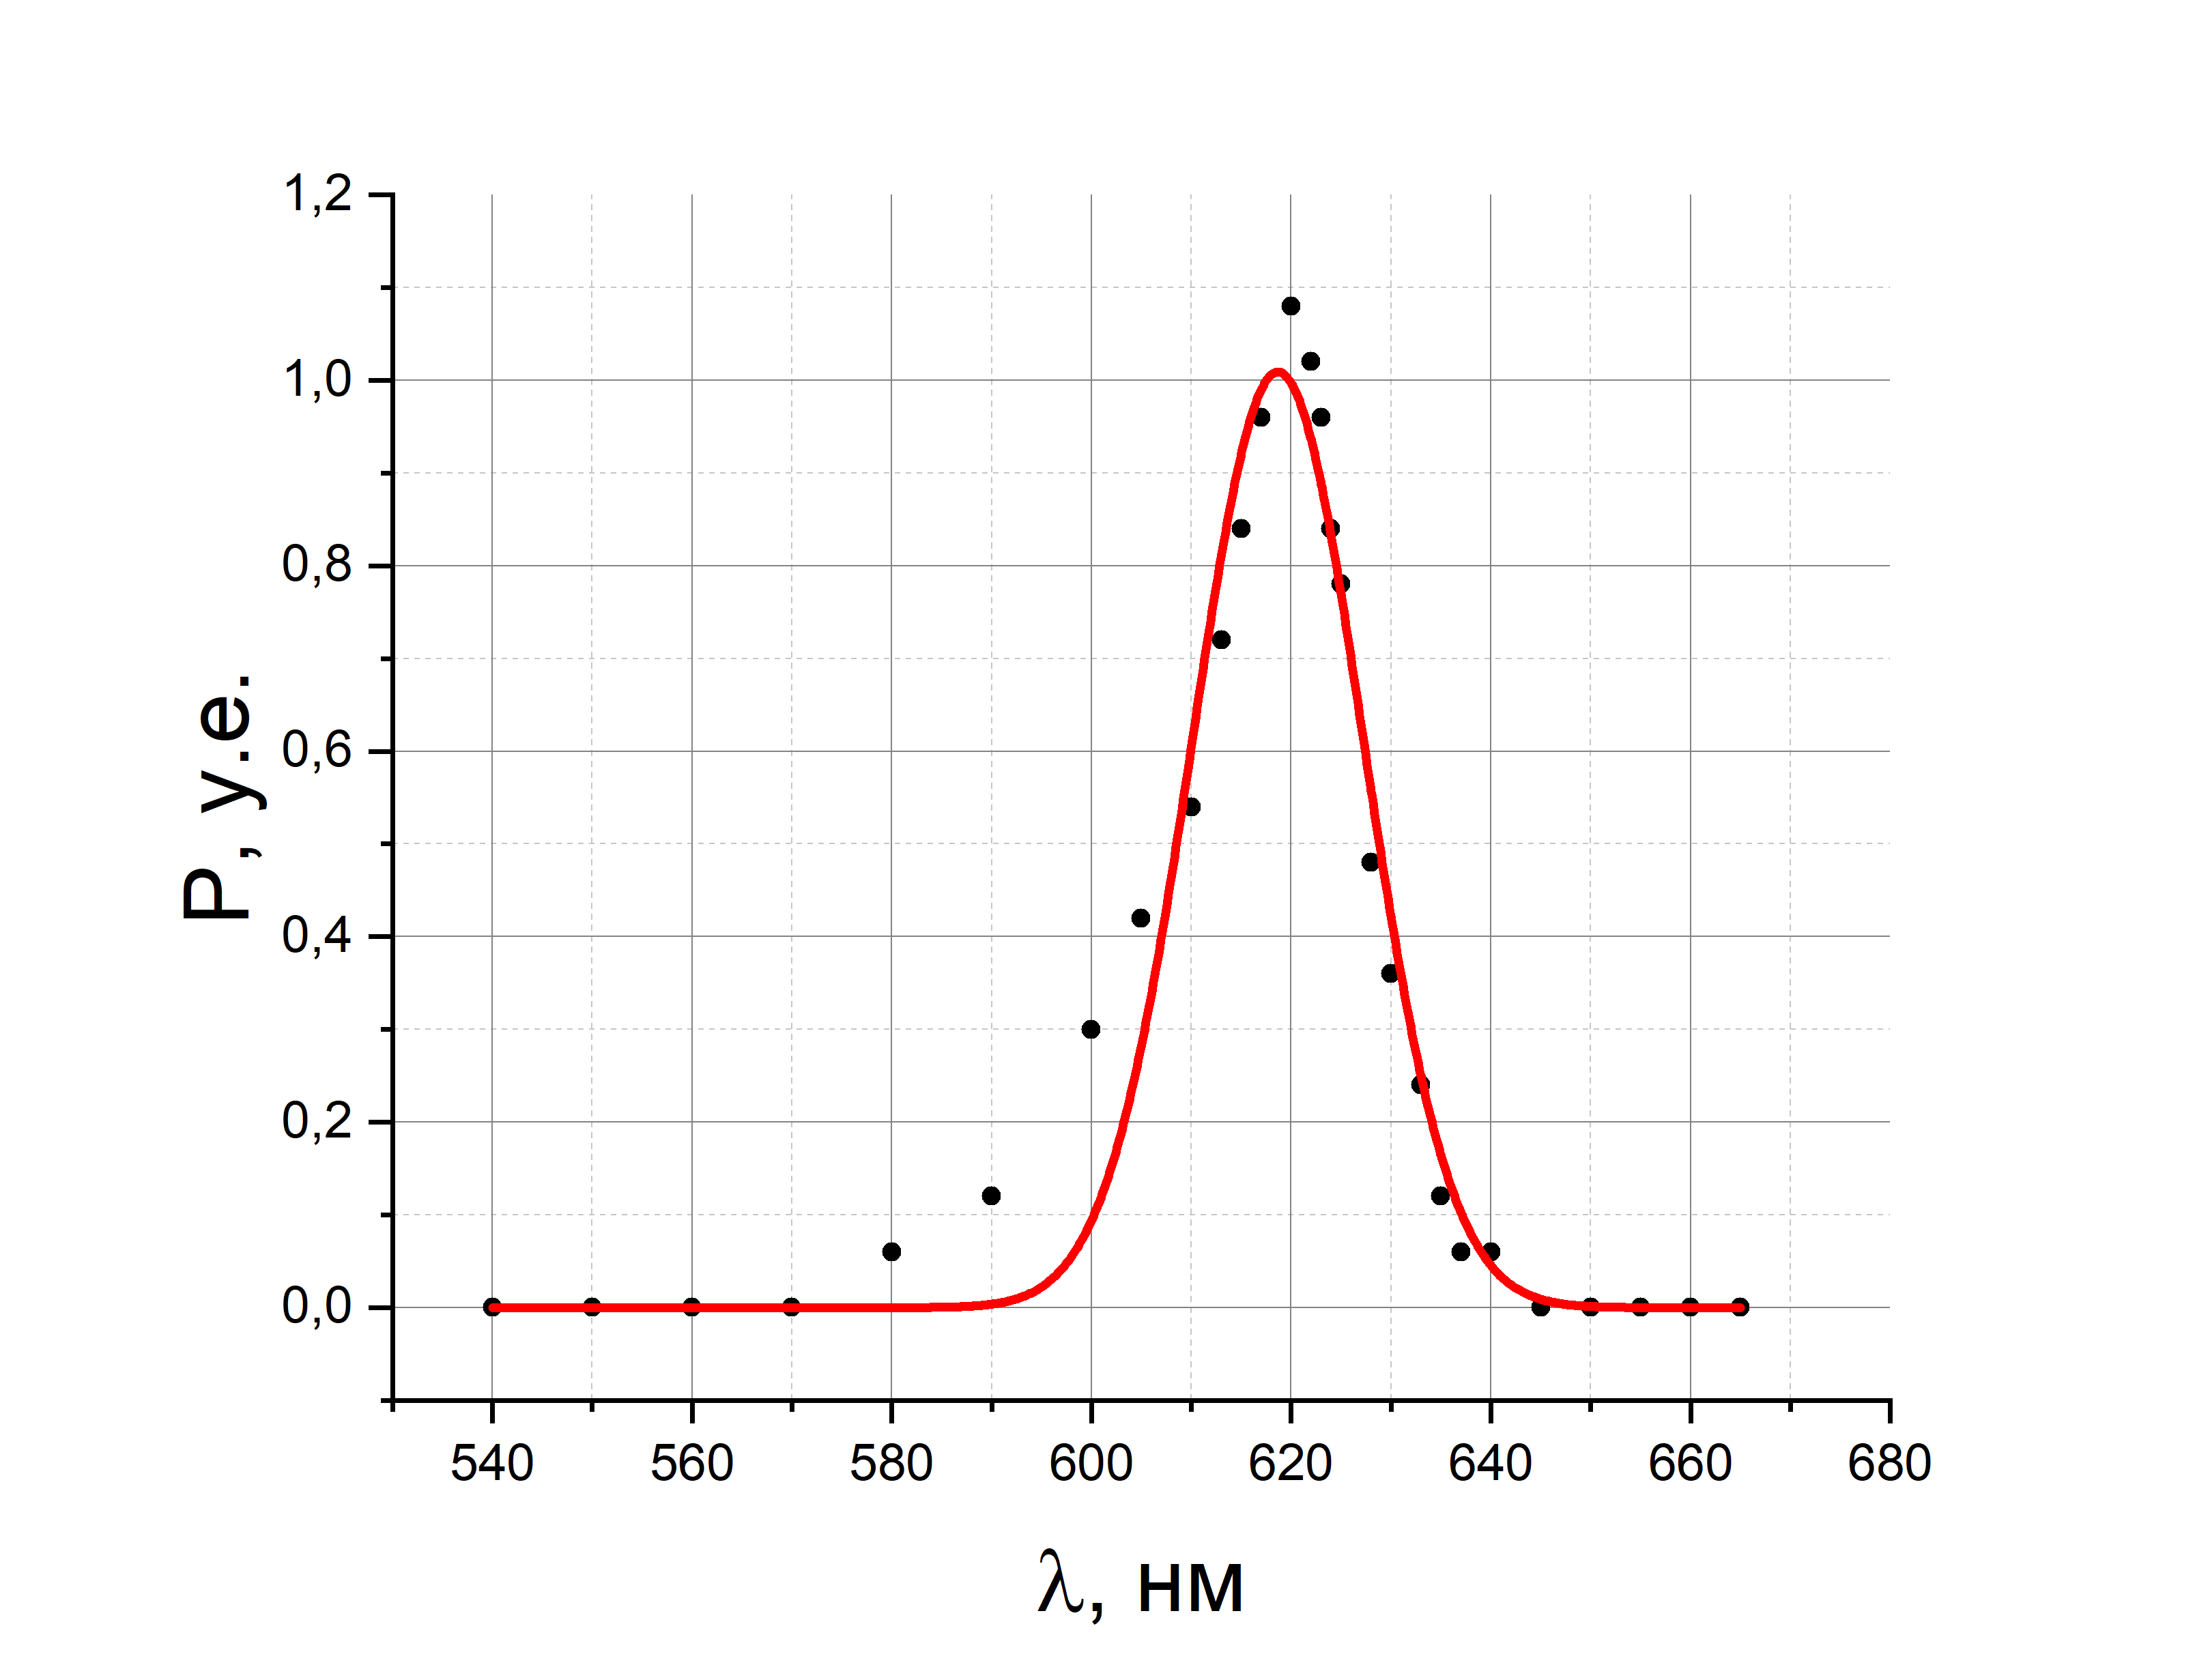
\includegraphics[width = 0.8\linewidth]{red}
	\caption{Спектральная характеристика для красного светодиода}
\end{figure}

\newpage

Длины волн, соответствующие пикам характеристик и полуширины линий занесем в таблицу:

\begin{table}[h]
\centering
\begin{tabular}{|c|c|c|}
\hline
                  & $\lambda$, нм & $\Delta \lambda$, нм \\ \hline
ПИЛ, I = 13,4 мА  & 651        & 12               \\ \hline
ПИЛ, I = 11 мА    & 651        & 12               \\ \hline
Синий, I = 4 мА   & 462        & 40               \\ \hline
Синий, I = 2,5 мА & 462        & 44               \\ \hline
Красный           & 619        & 34               \\ \hline
\end{tabular}
\end{table}

\section{Выводы}

\begin{enumerate}
	\item В результате работы были получены ватт-ваттные характеристики для ПИЛ и светодиодов разного цвета. Для ПИЛ была оценена пороговая мощность накачки $P_{\text{порог}} \approx 32$ мВт 
	\item Были также измерены спектральные характеристики ПИЛ и светодиодов для разных значений токов накачки. Из графиков видно, что изменение тока накачки приводит к изменению выходной мощности, как для лазера, так и для светодиода, причем профиль линии и длина волны не изменятся
\end{enumerate}

\newpage

\section{Приложение}

\begin{table}[h]
	\caption{Спектральная характеристика лазера для тока накачки $I = 13,4$ мА}
	\begin{tabular}{|c|c|c|c|c|c|c|c|c|c|c|c|c|c|}
	\hline
	$\lambda$, нм & 630 & 635 & 640 & 645 & 648 & 649 & 650 & 654  & 655 & 657 & 660 & 665 & 670 \\ \hline
	U,В        & 0   & 0   & 3   & 6,2 & 15  & 21  & 21  & 15,2 & 3,4 & 2,6 & 1,5 & 0,6 & 0   \\ \hline
	\end{tabular}
	\end{table}

\begin{table}[h]
	\caption{Спектральная характеристика лазера для тока накачки $I = 11$ мА}
	\begin{tabular}{|c|c|c|c|c|c|c|c|c|c|c|c|c|c|}
	\hline
	$\lambda$, нм & 640 & 645 & 647 & 650 & 651 & 652 & 653 & 654 & 655 & 656 & 657 & 660 & 665 \\ \hline
	U,В        & 0,3 & 0,8 & 1,6 & 3,4 & 3,8 & 3,4 & 2,8 & 2,2 & 1,5 & 1   & 0,8 & 0,4 & 0   \\ \hline
	\end{tabular}
	\end{table}

\begin{table}[h]
	\caption{Спектральная характеристика зеленого диода для тока накачки $I = 29$ мА}
	\begin{tabular}{|c|c|c|c|c|c|c|c|c|c|c|c|c|}
	\hline
	$\lambda$, нм & 450 & 455 & 460 & 465 & 470 & 480 & 485 & 490 & 495 & 500 & 505 & 510 \\ \hline
	U,В        & 0   & 0   & 0   & 0   & 0,2 & 0,4 & 0,6 & 0,8 & 1,2 & 1,4 & 1,8 & 1,9 \\ \hline
	\end{tabular}
	\end{table}

\begin{table}[h!]
	\caption{Спектральная характеристика красного диода для тока накачки $I = 17,5$ мА}
	\begin{tabular}{|c|c|c|c|c|c|c|c|c|c|c|c|c|c|c|c|c|c|c|c|c|c|c|c|c|c|c|c|c|}
		\hline
		$\lambda$, нм & 540 & 550 & 560 & 570 & 580  & 590  & 600 & 605  & 610  & 613  & 615  & 617   \\ \hline
		U,В        & 0   & 0   & 0   & 0   & 0,06 & 0,12 & 0,3 & 0,42 & 0,54 & 0,72 & 0,84 & 0,96\\ \hline
		$\lambda$, нм & 620  & 622  & 623  & 624  & 625  & 628  & 630  & 633  & 635  & 637  & 640  & 645 \\ \hline	
		U,В       & 1,08 & 1,02 & 0,96 & 0,84 & 0,78 & 0,48 & 0,36 & 0,24 & 0,12 & 0,06 & 0,06 & 0   \\ \hline
	\end{tabular}
\end{table}

\begin{table}[h!]
	\caption{Спектральная характеристика синего диода для тока накачки $I = 4$ мА}
	\begin{tabular}{|c|c|c|c|c|c|c|c|c|c|c|c|c|c|c|c|c|c|c|c|c|c|c|c|c|}
	\hline
	$\lambda$, нм & 410 & 420 & 430 & 440 & 450 & 455 & 457 & 458 & 460  & 462  & 464  & 466 & 468 & 470 \\ \hline
	U,В        & 0   & 0   & 0   & 0,9 & 4,2 & 7,8 & 9   & 9,6 & 10,2 & 10,8 & 10,6 & 9   & 7,8 & 6,8 \\ \hline
	$\lambda$, нм &473 & 476  & 483 & 486 & 490 & 495 & 500 & 505 & 510   \\ \hline
	U,В        &5,4 & 3,8 & 2,4 & 1,8 & 1,2 & 0,6 & 0,6 & 0   & 0 \\ \hline
	\end{tabular}
\end{table}

\begin{table}[h!]
	\caption{Спектральная характеристика синего диода для тока накачки $I = 2,5$ мА}
	\begin{tabular}{|c|c|c|c|c|c|c|c|c|c|c|c|c|c|c|c|c|c|c|c|c|c|c|c|c|c|c|}
	\hline
	$\lambda$, нм & 400 & 405 & 410 & 420 & 430 & 440 & 450 & 455 & 459 & 461 & 463 & 465 & 467 & 470 & 472 \\ \hline
	U,В        & 0   & 0   & 0   & 0   & 0   & 0,6 & 2,4 & 4,2 & 6   & 6,6 & 6,6 & 6   & 5,4 & 4,2 & 3,6 \\ \hline
	$\lambda$, нм & 474 & 476 & 479 & 481 & 484 & 487 & 489 & 492 & 495 & 500 & 505 \\ \hline
	U,В        & 3   & 3   & 2,4 & 1,8 & 1,8 & 1,2 & 0,6 & 0,6 & 0,6 & 0,3 & 0 \\ \hline   
	\end{tabular}
\end{table}

\newpage

\begin{table}[]
	\caption{Ватт-ваттная характеристика лазера}
	\begin{tabular}{|c|c|}
	\hline
	Pвх, мВт & Pвых, у.е. \\ \hline
	0        & 0,05       \\ \hline
	0,1722   & 0,05       \\ \hline
	2,1177   & 0,1        \\ \hline
	16,0776  & 1,29       \\ \hline
	22,1331  & 2,28       \\ \hline
	27,927   & 4,32       \\ \hline
	30,6404  & 7,31       \\ \hline
	31,1395  & 9,32       \\ \hline
	31,5735  & 13,08      \\ \hline
	31,9806  & 18,7       \\ \hline
	32,046   & 20,6       \\ \hline
	32,2204  & 27,8       \\ \hline
	32,4384  & 39,63      \\ \hline
	32,6128  & 48,1       \\ \hline
	32,7218  & 54,6       \\ \hline
	32,8962  & 65,3       \\ \hline
	33,3537  & 82,4       \\ \hline
	33,5727  & 104        \\ \hline
	34,364   & 130,6      \\ \hline
	34,958   & 172        \\ \hline
	35,398   & 197,95     \\ \hline
	35,9788  & 220,4      \\ \hline
	36,6639  & 260,6      \\ \hline
	37,3182  & 290,15     \\ \hline
	37,6956  & 311,35     \\ \hline
	37,9842  & 329,2      \\ \hline
	38,8689  & 369,35     \\ \hline
	39,5602  & 409,37     \\ \hline
	40,2752  & 440,91     \\ \hline
	40,95    & 465,47     \\ \hline
	41,8608  & 487        \\ \hline
	42,389   & 493,42     \\ \hline
	44,2389  & 501,6      \\ \hline
	46,7964  & 505,3      \\ \hline
	50,5108  & 515,3      \\ \hline
	60,5298  & 531,3      \\ \hline
	\end{tabular}
	\end{table}

\newpage

\begin{table}[]
	\caption{Ватт-ваттная характеристика зеленого диода}
	\begin{tabular}{|c|c|}
	\hline
	Pвх, мВт & Pвых, у.е. \\ \hline
	0        & 0,05       \\ \hline
	0,6      & 0,34       \\ \hline
	3,9932   & 1,94       \\ \hline
	9,0025   & 3,9        \\ \hline
	13,0384  & 5,28       \\ \hline
	19,0476  & 7,13       \\ \hline
	26,8011  & 9,2        \\ \hline
	34,456   & 11         \\ \hline
	45,2686  & 13,3       \\ \hline
	50,8389  & 14,37      \\ \hline
	58,7328  & 15,8       \\ \hline
	76,8421  & 19,24      \\ \hline
	89,775   & 20,95      \\ \hline
	92,295   & 21,34      \\ \hline
	106,88   & 23,63      \\ \hline
	112,378  & 24,42      \\ \hline
	120,528  & 25,75      \\ \hline
	137,61   & 28,3       \\ \hline
	151,302  & 30,02      \\ \hline
	166,788  & 31,88      \\ \hline
	181,104  & 33,33      \\ \hline
	\end{tabular}
	\end{table}

\newpage

\begin{table}[]
	
	\caption{Ватт-ваттная характеристика красного диода}
	\begin{tabular}{|c|c|}
	\hline
	Pвх, мВт & Pвых, у.е. \\ \hline
	0        & 0,05       \\ \hline
	0,076    & 0,06       \\ \hline
	2,128    & 1,03       \\ \hline
	4,147    & 2,09       \\ \hline
	5,6358   & 2,85       \\ \hline
	6,6865   & 3,38       \\ \hline
	8,7856   & 4,41       \\ \hline
	9,87     & 4,93       \\ \hline
	11,2896  & 5,6        \\ \hline
	12,8592  & 6,33       \\ \hline
	14,5882  & 7,12       \\ \hline
	16,0362  & 7,77       \\ \hline
	17,4833  & 8,37       \\ \hline
	18,4258  & 8,76       \\ \hline
	21,634   & 10,12      \\ \hline
	24,928   & 11,42      \\ \hline
	27,8306  & 12,55      \\ \hline
	32,1925  & 14,15      \\ \hline
	34,4736  & 14,97      \\ \hline
	35,64    & 15,42      \\ \hline
	38,1376  & 16,25      \\ \hline
	41,984   & 17,53      \\ \hline
	45,899   & 18,77      \\ \hline
	47,4129  & 19,22      \\ \hline
	48,8642  & 19,67      \\ \hline
	52,539   & 20,77      \\ \hline
	55,76    & 21,59      \\ \hline
	59,631   & 22,64      \\ \hline
	62,135   & 23,23      \\ \hline
	66,0982  & 24,21      \\ \hline
	70,4007  & 25,19      \\ \hline
	78,2781  & 26,82      \\ \hline
	88,29    & 28,66      \\ \hline
	\end{tabular}
	\end{table}

\newpage

\begin{table}[]
	\caption{Ватт-ваттная характеристика синего диода}
	\begin{tabular}{|c|c|}
	\hline
	Pвх, мВт & Pвых, у.е. \\ \hline
	0        & 0,05       \\ \hline
	0,3036   & 0,27       \\ \hline
	0,8976   & 0,96       \\ \hline
	1,232    & 1,36       \\ \hline
	1,8166   & 2,06       \\ \hline
	2,5481   & 2,87       \\ \hline
	3,2538   & 3,65       \\ \hline
	3,8048   & 4,2        \\ \hline
	4,7677   & 5,14       \\ \hline
	5,4208   & 5,75       \\ \hline
	5,976    & 6,26       \\ \hline
	6,6789   & 6,85       \\ \hline
	7,6782   & 7,65       \\ \hline
	8,4456   & 8,27       \\ \hline
	9,744    & 9,24       \\ \hline
	10,9516  & 10,04      \\ \hline
	11,4904  & 10,45      \\ \hline
	12,3405  & 10,99      \\ \hline
	13,5725  & 11,79      \\ \hline
	14,651   & 12,45      \\ \hline
	15,6368  & 13         \\ \hline
	16,52    & 13,52      \\ \hline
	17,424   & 14,01      \\ \hline
	18,942   & 14,84      \\ \hline
	20,1804  & 15,45      \\ \hline
	22,0759  & 16,43      \\ \hline
	22,5593  & 16,66      \\ \hline
	\end{tabular}
	\end{table}

\end{document}
